\subsection{Phân hệ Xác thực và Quản lý Phiên (Auth Module)}
\label{subsec:module_auth}

\subsubsection{Mô tả Nghiệp vụ và Yêu cầu Chức năng}
Phân hệ Xác thực và Quản lý Phiên đóng vai trò là cửa ngõ an ninh cho toàn bộ ứng dụng di động MyHCMUT, chịu trách nhiệm xác thực danh tính người dùng qua máy chủ xác thực tập trung của Nhà trường (HCMUT CAS SSO) hoặc tài khoản nội bộ, quản lý phiên làm việc đa miền qua cơ chế Dual-Token, tự động làm mới phiên ngầm (Silent Refresh) và cung cấp giải pháp One-Time Ticket SSO cho phép người dùng mở các phân hệ Web chuyên sâu mà không cần đăng nhập lại:

\begin{itemize}
    \item \textbf{Quản lý Phiên làm việc Đa miền:} Lưu trữ chuỗi Access Token và Refresh Token qua \texttt{MultiDomainTokenManager} sử dụng vùng nhớ riêng biệt của ứng dụng trên \texttt{SharedPreferences} kết hợp bộ đệm In-Memory truy xuất tức thì $O(1)$, hỗ trợ xóa sạch dữ liệu khi đăng xuất.
    \item \textbf{Làm mới phiên làm việc ngầm (Silent Refresh):} Tự động bắt lỗi HTTP 401 Unauthorized tại \texttt{MultiDomainAuthInterceptor} để kích hoạt luồng làm mới token ngầm mà không làm gián đoạn trải nghiệm người dùng.
    \item \textbf{Cơ chế One-Time Ticket SSO cho Web App:} Cung cấp cơ chế cấp vé dùng một lần (TTL 60s, Single-use trên Redis) cho phép ứng dụng di động mở các phân hệ Web mở rộng qua WebView/InAppBrowser an toàn, không truyền JWT trực tiếp trên URL.
\end{itemize}

\subsubsection{Đặc tả Ca sử dụng (Use Cases)}

\begin{table}[H]
\centering
\renewcommand{\arraystretch}{1.2}
\small
\begin{tabularx}{\textwidth}{|L{3.2cm}|Y|}
\hline
\textbf{Mã Ca sử dụng} & \textbf{UC\_AUTH\_01: Đăng nhập Hệ thống và Quản lý Phiên Đa miền} \\
\hline
\textbf{Tác nhân} & Toàn bộ cán bộ, giảng viên, nhân viên Nhà trường \\
\hline
\textbf{Tiền điều kiện} & Cán bộ có tài khoản HCMUT SSO hoặc tài khoản nội bộ còn hoạt động. \\
\hline
\textbf{Hậu điều kiện} & Cán bộ được cấp Access Token dùng chung (Shared JWT), lưu trữ an toàn và nạp hồ sơ người dùng. \\
\hline
\textbf{Luồng sự kiện chính} & 
1. Người dùng mở ứng dụng MyHCMUT, chọn phương thức đăng nhập (CAS SSO hoặc Mật khẩu). \newline
2. Người dùng nhập thông tin xác thực và nhấn \textit{``Đăng nhập''}. \newline
3. Ứng dụng gửi yêu cầu tới máy chủ xác thực \texttt{myhcmut-be} qua endpoint \texttt{POST /api/auth/login}. \newline
4. Máy chủ xác thực thông tin, cấp cặp token (\texttt{accessToken}, \texttt{refreshToken}) chứa các thông tin định danh (\texttt{shcc}, \texttt{maDonVi}, \texttt{roles}, \texttt{permissions}). \newline
5. Ứng dụng lưu trữ token vào \texttt{MultiDomainTokenManager}, kích hoạt \texttt{authStateProvider} và điều hướng vào màn hình chính Dashboard. \\
\hline
\textbf{Luồng ngoại lệ} & Nếu thông tin xác thực không chính xác $\rightarrow$ Hệ thống hiển thị thông báo lỗi và yêu cầu nhập lại; nếu tài khoản bị khóa $\rightarrow$ từ chối đăng nhập. \\
\hline
\end{tabularx}
\caption{\textit{Đặc tả Ca sử dụng UC\_AUTH\_01: Đăng nhập Hệ thống và Quản lý Phiên}}
\label{tab:uc_auth_01}
\end{table}

\begin{table}[H]
\centering
\renewcommand{\arraystretch}{1.2}
\small
\begin{tabularx}{\textwidth}{|L{3.2cm}|Y|}
\hline
\textbf{Mã Ca sử dụng} & \textbf{UC\_AUTH\_02: One-Time Ticket SSO Chuyển tiếp sang Web App} \\
\hline
\textbf{Tác nhân} & Cán bộ, giảng viên có nhu cầu mở phân hệ Web phụ trợ từ Mobile \\
\hline
\textbf{Tiền điều kiện} & Cán bộ đã đăng nhập hợp lệ trên ứng dụng di động MyHCMUT, có chuỗi \texttt{accessToken} hợp lệ. \\
\hline
\textbf{Hậu điều kiện} & Ứng dụng Web mở ra trên In-App WebView với phiên làm việc đã được xác thực tự động (không cần nhập lại mật khẩu). \\
\hline
\textbf{Luồng sự kiện chính} & 
1. Cán bộ nhấn chọn một tính năng chuyên sâu cần mở giao diện Web trên ứng dụng Mobile (ví dụ: giải trình trễ hạn, thẩm định danh mục lý lịch chuyên sâu). \newline
2. Ứng dụng Mobile gọi API \texttt{POST /api/auth/sso/generate-ticket} gửi kèm thông tin định danh và đích đến (\texttt{targetApp: 'hrm-fe'}). \newline
3. Backend sinh vé ngẫu nhiên an toàn bằng bộ tạo số ngẫu nhiên mật mã học gồm 32 bytes ngẫu nhiên mã hóa hex (chuỗi 64 ký tự hex), lưu vào Redis dưới khóa \texttt{sso:ticket:<ticket>} với TTL 60 giây (\texttt{SET EX 60}) và trả về cho Mobile. \newline
4. Mobile mở In-App WebView tải URL đích đính kèm vé: \texttt{https://domain/feature?ticket=<hex64>}. \newline
5. Web Frontend phát hiện tham số \texttt{ticket} trong URL query, lập tức trích xuất và gọi \texttt{POST /api/auth/sso/consume-ticket}. \newline
6. Backend thực hiện đọc và xóa vé nguyên tử trên Redis bằng lệnh \texttt{GETDEL} (hoặc Lua script tương đương), cấp Session Cookie (\texttt{connect.sid}) với các cờ bảo vệ \texttt{HttpOnly; SameSite=Lax; Secure} cho Web Frontend. \newline
7. Web Frontend làm sạch tham số vé trên thanh địa chỉ thông qua \texttt{window.history.replaceState} để chống lộ lọt vé qua lịch sử duyệt web hoặc header Referer, sau đó kết xuất trực tiếp màn hình chức năng. \\
\hline
\textbf{Luồng ngoại lệ} & Nếu vé quá hạn 60 giây hoặc đã bị tiêu thụ trước đó $\rightarrow$ Lệnh \texttt{GETDEL} trả về rỗng $\rightarrow$ Backend trả về HTTP 401 Unauthorized $\rightarrow$ Web App chuyển hướng an toàn về màn hình đăng nhập chuẩn. \\
\hline
\end{tabularx}
\caption{\textit{Đặc tả Ca sử dụng UC\_AUTH\_02: One-Time Ticket SSO sang Web App}}
\label{tab:uc_auth_02}
\end{table}

\subsubsection{Phân tích An toàn Mô hình Đe dọa STRIDE cho Cầu nối SSO (SSO Bridge)}

Cơ chế cầu nối SSO giữa ứng dụng Native Mobile và In-App WebView được kiểm toán an ninh nghiêm ngặt dựa trên mô hình đe dọa STRIDE (Spoofing, Tampering, Repudiation, Information Disclosure, Denial of Service, Elevation of Privilege):

\begin{table}[H]
\centering
\small
\renewcommand{\arraystretch}{1.25}
\begin{tabularx}{\textwidth}{|>{\RaggedRight\arraybackslash\small}p{2.8cm}|>{\RaggedRight\arraybackslash\small}p{4.2cm}|Y|}
\hline
\textbf{Mối đe dọa STRIDE} & \textbf{Nguy cơ Tiềm ẩn} & \textbf{Biện pháp Giảm thiểu Kỹ thuật} \\
\hline
\textbf{Spoofing (Giả mạo)} & Kẻ tấn công giả danh người dùng gửi request xin cấp vé SSO. & Backend bắt buộc xác thực \texttt{Bearer JWT} hợp lệ trước khi sinh vé; chỉ cấp vé cho đúng định danh \texttt{shcc} đang đăng nhập. \\
\hline
\textbf{Tampering (Sửa đổi)} & Chỉnh sửa tham số vé hoặc URL chuyển tiếp trên đường truyền. & Bắt buộc mã hóa toàn bộ kênh truyền qua HTTPS/TLS; vé có entropy cực cao (256-bit entropy / 64 ký tự hex) không thể đoán trước hoặc làm giả. \\
\hline
\textbf{Information Disclosure (Lộ lọt thông tin)} & Vé bị lộ qua nhật ký truy cập mạng (Access Logs), header Referer hoặc lịch sử trình duyệt. & Rút ngắn thời gian sống của vé (TTL 60s); Web Frontend thực thi ngay \texttt{window.history.replaceState} xóa sạch tham số \texttt{ticket} khỏi URL. \\
\hline
\textbf{Repudiation \& Elevation of Privilege} & Tấn công phát lại (Replay Attack): Kẻ tấn công chặn bắt vé và dùng lại để chiếm đoạt phiên. & Tiêu thụ vé nguyên tử với Redis \texttt{GETDEL}; vé chỉ có giá trị sử dụng duy nhất một lần (Single-use). Nếu gọi lại lần 2, hệ thống từ chối ngay lập tức (đã kiểm chứng qua 46 ca kiểm thử SSO). \\
\hline
\end{tabularx}
\caption{\textit{Ma trận Phân tích An ninh STRIDE cho Cầu nối One-Time Ticket SSO}}
\label{tab:sso_stride}
\end{table}

\subsubsection{Biểu đồ Tuần tự (Sequence Diagrams)}

\begin{figure}[H]
    \centering
    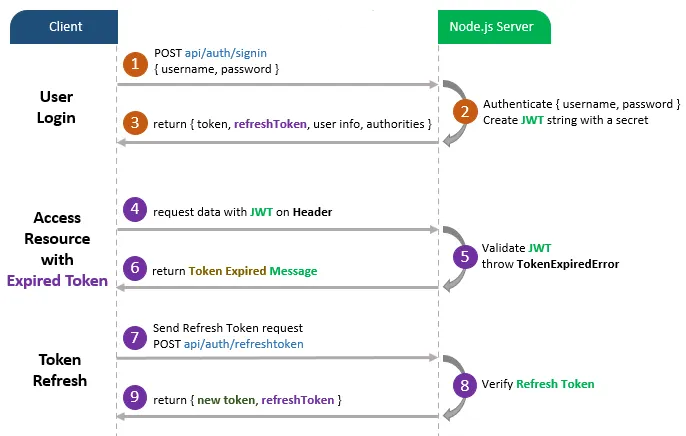
\includegraphics[width=0.85\linewidth]{img/uml/seq_login_token.png}
    \caption{\textit{Biểu đồ Tuần tự Đăng nhập SSO và Phân phối Token Dùng chung}}
    \label{fig:seq_auth_login}
\end{figure}

Biểu đồ hình \ref{fig:seq_auth_login} mô tả chi tiết quy trình người dùng xác thực với máy chủ đăng nhập tập trung, cơ chế phân phối chuỗi JWT dùng chung (\texttt{Shared JWT}) được ký bởi khóa bí mật \texttt{AUTH\_JWT\_SECRET}, cho phép các backend \texttt{hrm-be} và \texttt{ioffice-be} xác thực cục bộ độc lập với độ trễ dưới 5ms. Bên cạnh đó, toàn bộ logic sinh vé, tiêu thụ vé nguyên tử và xử lý lỗi đã được bảo vệ bởi bộ 46 ca kiểm thử tự động (\texttt{sso\_*.unit.test.ts}) đạt tỷ lệ vượt qua 100\%.
